\section{Curvature-driven tracking theory}
\label{sec:tracking-theory}

This section proves a finite-sample comparison theorem for perturbed WGF.
The central object is the curvature propagator \(G_\kappa^Y(t,s)\), defined below.
It transports an error created at time \(s\) to time \(t\), discounting or
amplifying it according to the curvature accumulated after its creation.

\subsection{Curvature-response factors}
\label{subsec:curvature-budgets}

\begin{definition}[Curvature-response factors]
\label{def:curvature-responses}
Let  $\HessianMatrices_t^Y$ denote the empirical discretization of $\mathcal{H}_{\mu_t}$ along the
reference particles, acting on the indexed particle space $(\mathbb R^d)^N$:
\begin{equation}
    \HessianMatrices_t^Y\coloneq
    \left\{
    \frac{1}{N}
    \nabla_W^2 F\!\left(\mu_t,Y^i_t,Y^j_t\right)
    + \delta_{ij}\nabla_x\nabla_W F\!\left(\mu_t,Y^i_t\right)\in \R^{d\times d}\right\}_{i,j=1}^N.
\end{equation}
We define the sampled curvature by
\begin{equation}
    \kappa^{Y,N}_t := \lambda_{\min}(\HessianMatrices^Y_t) \coloneq 
    \inf_{\mathbf v \in (\R^d)^N, \norm{\mathbf v}_2=1}
    \langle \mathbf v,\HessianMatrices^Y_t \mathbf v\rangle
    \label{eq:curvature-main}
\end{equation}
Positive \(\kappa_t^{Y,N}\) corresponds to instantaneous contraction of the
linearized discrepancy, while negative \(\kappa_t^{Y,N}\) corresponds to local
expansion.  This is the same role played by a local strong-convexity parameter in
ordinary gradient descent, except that here the parameter may change sign along
the trajectory. For example, $F(\mu)=\int \frac{\norm{x}^2}{2}\,\dd\mu$ implies $\HessianMatrices_t^Y = \boldsymbol{I}_{dN}$ and $\kappa_t^{Y,N} = 1>0$.

On any reference path satisfying
\(\int_0^T|\kappa_u^{Y,N}|\,\dd u<\infty\), we define the continuous
curvature-response factor
\[
    \mathfrak C_t^Y
    \coloneq 
    \int_0^t
    G_\kappa^Y(t,s)
    \dd s ,\quad G_\kappa^Y(t,s)
    \coloneq 
    \exp\left\{-\int_s^t \kappa_u^{Y,N}\,\dd u\right\},
    \qquad 0\le s\le t
\]
and the jump curvature-response factor
\[
    \mathfrak J_t^Y
    :=
    \sum_{\ell=1}^{L_t}
    \eta_\ell
    G_\kappa^Y(t,t_\ell)
    ,\quad L_t:=\#\{\ell:t_\ell\le t\}.
\]
\end{definition}
\begin{remark}[Conditioning used below.]
Let \(\mathcal G_{\mathrm{pop}}\) be the sigma-field generated by the population
Gaussian fields and the prescribed jump schedule. Conditional on
\(\mathcal G_{\mathrm{pop}}\), the reference particles are i.i.d. with law
\(\mu_t\), while the finite-dimensional coupling vectors
\(\mathbf g_\ell^N\) are not included in this conditioning; see
\Cref{subsec:auxiliary-particles}.
\end{remark}

\subsection{Main theorem}
\label{subsec:main-theorem}

We now quantify how curvature controls the accumulation of drift
fluctuations and jump mismatches over a growing horizon, under the following
assumptions:
\begin{itemize}[leftmargin=1.25em,itemsep=0pt,topsep=2pt,parsep=0pt]
    \item a structured moment representation of \(F\), with weighted smoothness
    controlling its drift and Hessian
    (\Cref{assumption-main-general-moment-smooth-compressed});
    \item uniform particle moments, branchwise Lipschitz paths, and the stated
    non-spikiness bound for the paired errors
    (\Cref{assumption-main-coupled-particle-regularity}); and
    \item a prescribed deterministic common schedule and the population-first
    Gaussian coupling (\Cref{assumption-main-jump-time}).
\end{itemize}
Under these conditions, we obtain the following comparison, valid
simultaneously for all \(t\in[0,T]\).

\begin{theorem}[Particle and objective tracking along controlled-curvature paths]
\label{theorem-main-r_t}
Assume \Cref{assumption-main-general-moment-smooth-compressed,assumption-main-coupled-particle-regularity,assumption-main-jump-time}, with fixed structural
parameters. Fix $\upsilon\ge0$, $\zeta>0$ with $\upsilon+\zeta<1/4$, and constants $C_p,C_0,L_0>0$.
Let $T\le N^{1/4-\upsilon-\zeta}$, $p\in[N^{-C_p},1)$, and use a prescribed deterministic
schedule with at most $L_0$ jumps and amplitudes $0\le\eta_\ell\le C_0$.
For brevity, write
$\Xi_{N,T,p}:=N(e+T)/p$.
For each \(N,T,p\), there is an event
$\Omega_p=\Omega_{N,T,p}$, independent of \(\varepsilon\), with probability at
least $1-p$. For every $\varepsilon>0$ and all sufficiently large $N$, the
following holds on $\Omega_p$. Suppose that the realized reference path satisfies
\[
\int_0^T|\kappa_t^{Y,N}|\,\dd t<\infty,\qquad
\sup_{t\le T}\mathfrak C_t^Y\le C_0N^\upsilon(1+T),\qquad
\sup_{t\le T}\mathfrak J_t^Y\le C_0N^\upsilon.
\]
Then, with $r_t=(N^{-1}\sum_{i=1}^N
\|X_t^i-Y_t^i\|_{\mathbb R^d}^2)^{1/2}$, simultaneously for $t\in[0,T]$,
\begin{equation}
\label{eq:objective-tracking-bound}
\begin{aligned}
&r_t\vee|F(\rho_{\mathbf X_t})-F(\mu_t)|\\
&\quad\le C_\varepsilon\Xi_{N,T,p}^{\varepsilon}
\left[(N^{-1/2}+T/N)(1+\mathfrak C_t^Y)
 +(N^{-1/4}+\sqrt{T/N})\mathfrak J_t^Y\right].
\end{aligned}
\end{equation}
Here $\vee$ denotes the maximum. The constants may depend on the fixed
parameters, including $\upsilon,\zeta,C_p,C_0,L_0$.
\end{theorem}

We also report numerical sanity checks of non-spikiness and adaptive PWGF in \Cref{sec:numerical-sanity}.

\noindent\textbf{Curvature determines how long finite-sample errors persist.}
The ODE residual has scale \(N^{-1/2}+T/N\), while the jump mismatch has scale
\(N^{-1/4}+\sqrt{T/N}\), apart from the common subpolynomial factor
\(C_\varepsilon\Xi_{N,T,p}^{\varepsilon}\). The \(T/N\) and
\(\sqrt{T/N}\) terms arise from controlling the residuals over the entire
interval \([0,T]\); under
\(T\le N^{1/4-\upsilon-\zeta}\), they are dominated by \(N^{-1/2}\) and \(N^{-1/4}\),
respectively. These scales are then weighted by the actual curvature
propagator \(G_\kappa^Y\): \(\mathfrak C_t^Y\) accumulates errors generated
continuously, whereas \(\mathfrak J_t^Y\) propagates jump mismatches. Keeping this
propagator avoids replacing the accumulated curvature by a worst-case bound
that can grow exponentially in \(T\). Positive curvature makes past errors
decay, while negative curvature can preserve or amplify them
(\Cref{fig:curvature-response}). A jump mismatch may therefore dominate just
after a perturbation and later be forgotten, whereas continuous errors are
generated throughout the flow.

The following example makes this curvature-dependent tracking bound concrete.

\begin{example}[Growing-horizon tracking in a variance-plus-cosine model]
\label{ex:variance-cosine-curvature-recovery}
In dimension one, consider the model in \Cref{subsec:canonical-variance-cosine},
\[
 F(\mu)=\frac a2\operatorname{Var}(\mu)+\beta\cos(\pi m_\mu),
 \qquad m_\mu=\int x\,\mu(dx),\qquad a,\beta>0.
\]
Take a fixed bounded mean-zero initial law and one prescribed Gaussian jump
at a fixed time $\tau>0$ with fixed amplitude $\eta>0$, independently of $N$.
Writing $m_t=m_{\mu_t}$ and setting $T=N^{1/8}$,
\Cref{prop:canonical-model-assumptions} gives an event of probability at least
$1-N^{-1/16}$ on which
\Cref{lem:canonical-response-control,eq:canonical-sampled-curvature,eq:canonical-response-bounds} give
\[
 \kappa_t^{Y,N}=\min\{a,-\beta\pi^2\cos(\pi m_t)\},
 \qquad
 \sup_{0\le t\le T}(\mathfrak C_t^Y+\mathfrak J_t^Y)\le CN^{1/16}.
\]
\Cref{theorem-main-r_t} then gives, on the same event,
\[
 \sup_{0\le t\le T}
 \left[r_t+\left|F(\rho_{\mathbf X_t})-F(\mu_t)\right|\right]
 \le C_\varepsilon N^{-3/16+\varepsilon}.
\]
The bounds hold for each fixed $\varepsilon>0$ and sufficiently large $N$,
with fixed model parameters.
\end{example}

\begin{figure}[!h]
    \centering
    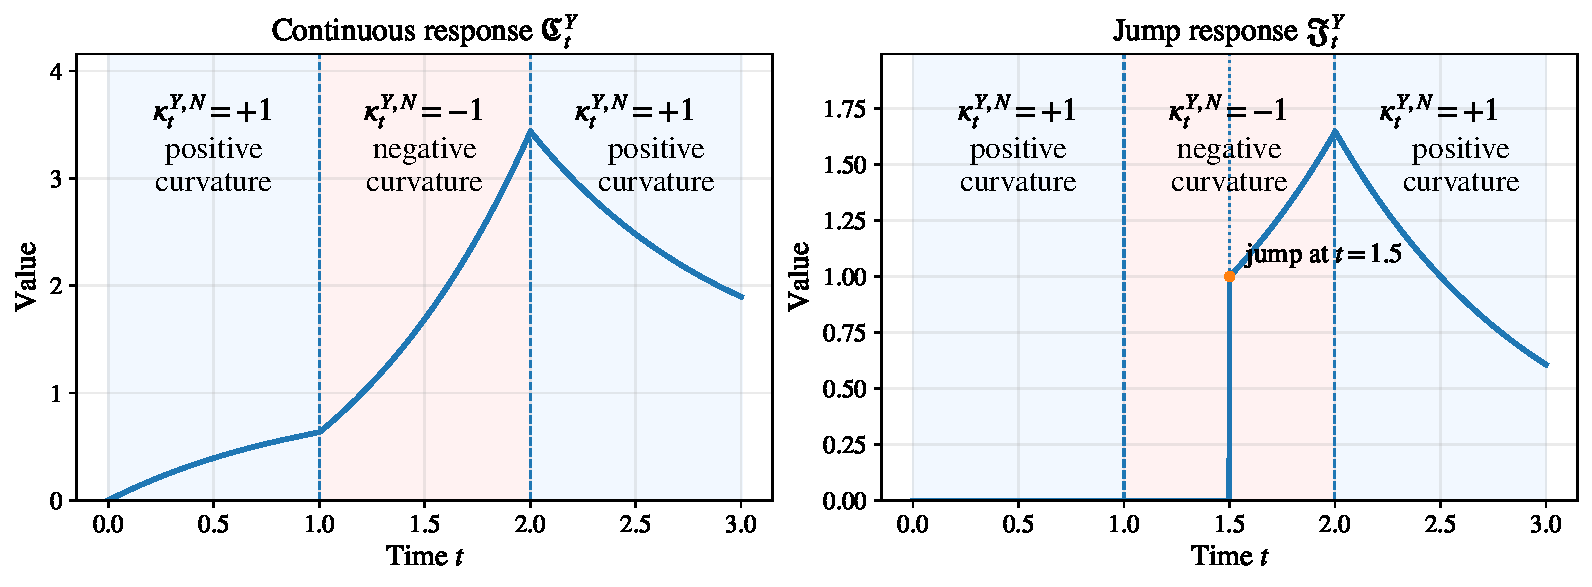
\includegraphics[width=0.7\linewidth]{sections/curvature_response_horizontal.pdf}
    \caption{
    Illustration of the curvature-response factors in the tracking bound. We assume that $\kappa_t^{Y,N} = 1$ (positive curvature) if $t\in[0,1)\cup[2,3]$ and $\kappa_t^{Y,N} = -1$ (negative curvature) if $t\in[1,2)$.
    The factor \(\mathfrak C_t^Y\) measures the remaining effect of unit ODE forcing,
    while \(\mathfrak J_t^Y\) records a unit jump at \(t=1.5\), followed by
    amplification under negative curvature and decay under positive curvature.
    }
    \label{fig:curvature-response}
\end{figure}
